\subsection{Resultate \label{subsec:cmb:results}}

Die Resultate der Analyse bestätigen die bereits bekannten Resultate der ESA 
Planck Mission. Die Resultate mussten allerdings jeweils mit einem konstanten 
Faktor angepasst werden.

\subsubsection{2K Auflösung}

Das 2K aufgelöste Bild lässt ein maximales $l$ von 1000 zu. Wie man in 
Abbildung~\ref{fig:cmb-power-spec-900} sehen kann, gibt es bei rund $l = 200$ 
ein Maximum. Die $C_l$-Werte mussten zudem mit einem Faktor von 
$\frac{1}{1085}$ skaliert werden, damit das Maximum in etwa mit demjenigen aus 
Abbildung~\ref{fig:planck_spectrum} vergleichbar ist.

\begin{figure}
	\centering
	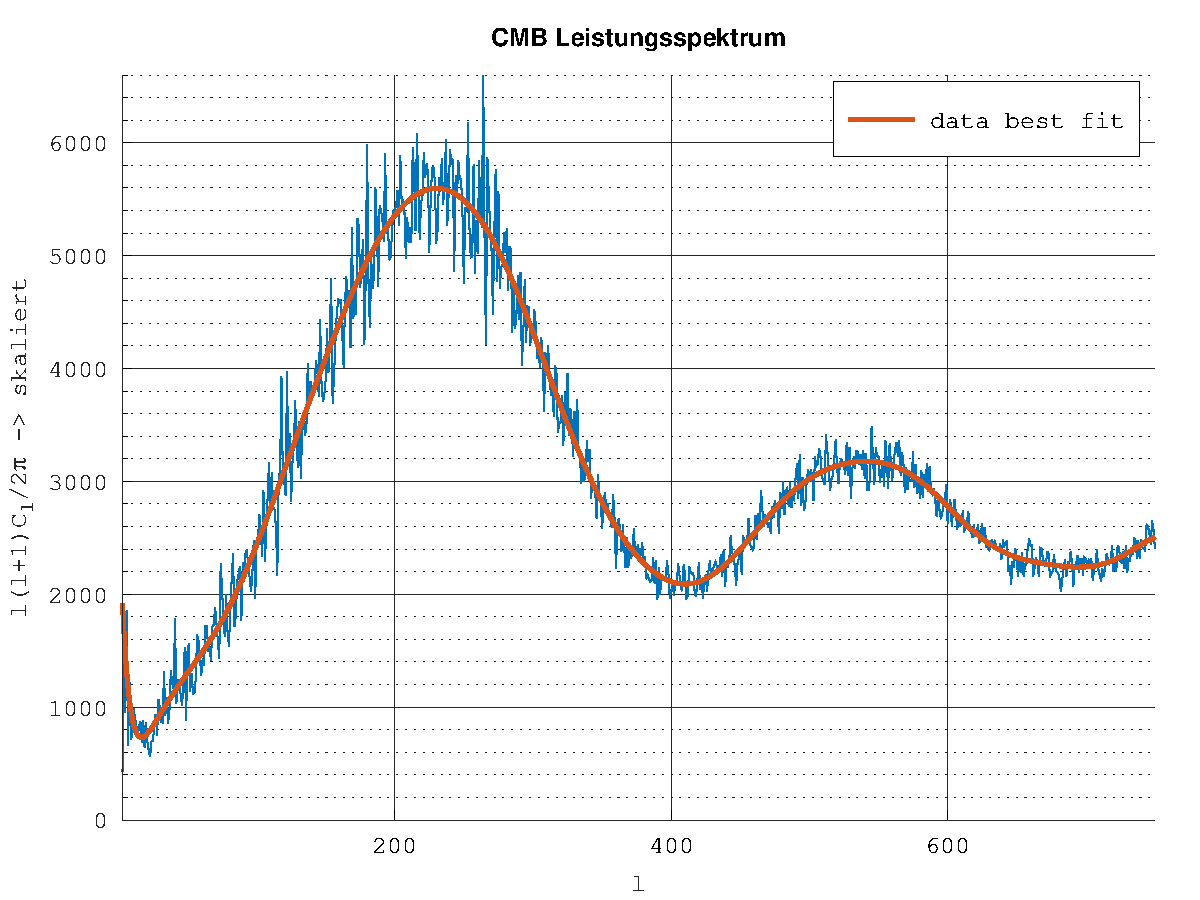
\includegraphics[width=\linewidth]{cmb/data/2k900-500.pdf}
	\caption{Leistungsspektrum berechnet bis zu $l = 900$. Grundlage für die 
		Berechnung ist das 2K aufgelöste Bild der ESA Planck Mission.}
	\label{fig:cmb-power-spec-900}
\end{figure}

\subsubsection{4K Auflösung}

Das 4K Bild lässt bereits ein maximales $l$ von 2000 zu. 
Abbildung~\ref{fig:cmb-power-spec-1600} zeigt deutlich, die Übereinstimmung mit 
den Planck Auswertungen. Der Skalierungsfaktor der erhaltenen Daten beträgt 
$\frac{1}{1980}$.

\begin{figure}
	\centering
	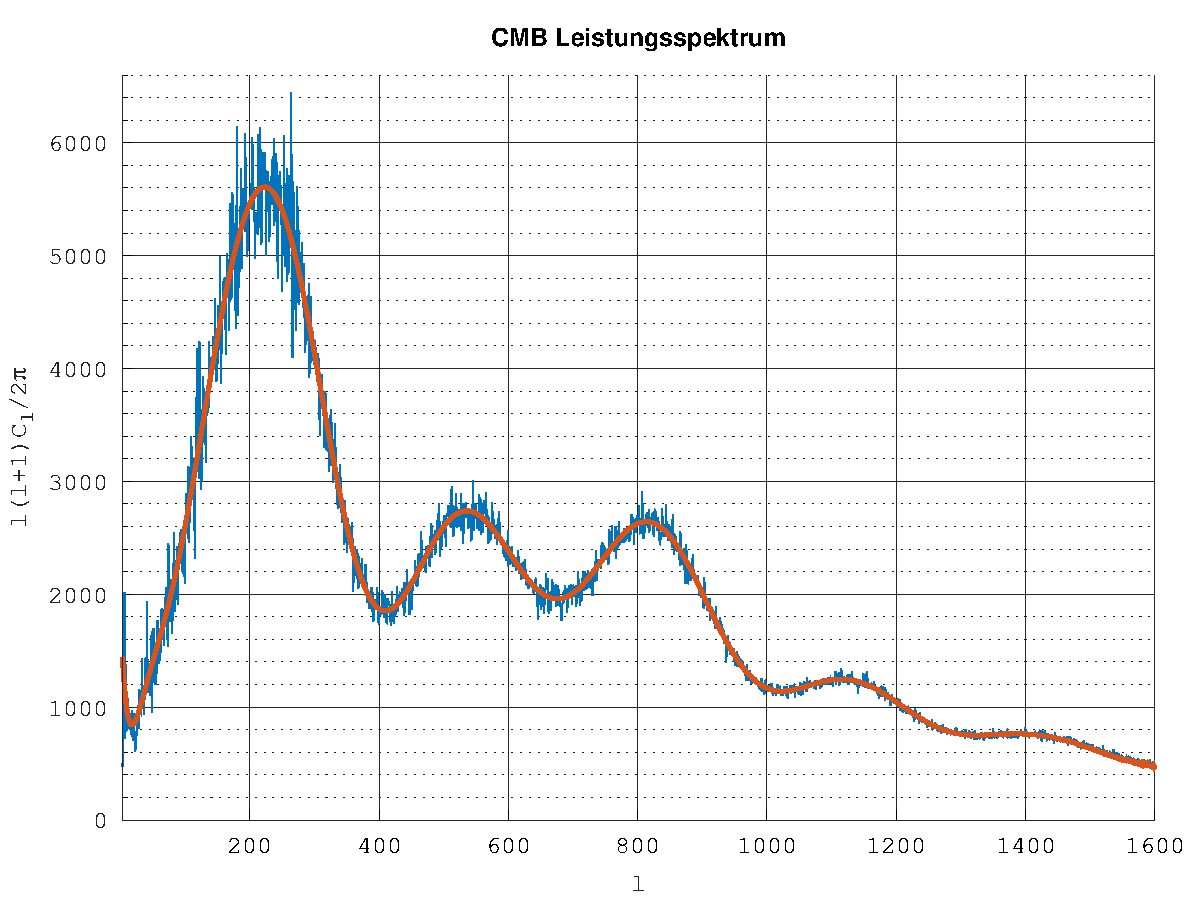
\includegraphics[width=\linewidth]{cmb/data/4k1800-500.pdf}
	\caption{Leistungsspektrum berechnet bis zu $l = 1600$. Grundlage für die 
		Berechnung ist das 4K aufgelöste Bild der ESA Planck Mission.}
	\label{fig:cmb-power-spec-1600}
\end{figure}

\subsubsection{12K Auflösung}

Das 12K Bild ist nicht direkt online erhältlich, sondern nur auf Anfrage, was 
bei einer Bildgrösse von fast 180 Megabyte durchaus verständlich ist. Die 
Bildgrösse hat auch Auswirkungen auf die Analyse. So wird mit der derzeitigen 
Library Implementation fast 80 Gigabyte Arbeitsspeicher benötigt um eine 
Analyse mit maximalem $l$ von 2500 durchzuführen. Der ausgegeben Werte müssen 
mit $\frac{1}{6900}$ skaliert werden um vergleichbar zu sein. Es zeigt sich, 
dass die Resultate bei grösseren $l$ nicht mehr ganz übereinstimmen. Dies liegt 
aber vermutlich an der Transformationsfunktion die für dieses Bild nicht mehr 
ganz passt. Trotzdem zeigen sich auch hier die Maximalstellen bei den gleichen 
$l$-Werten wie bereits in den Resultaten der ESA Planck Mission.

\begin{figure}
	\centering
	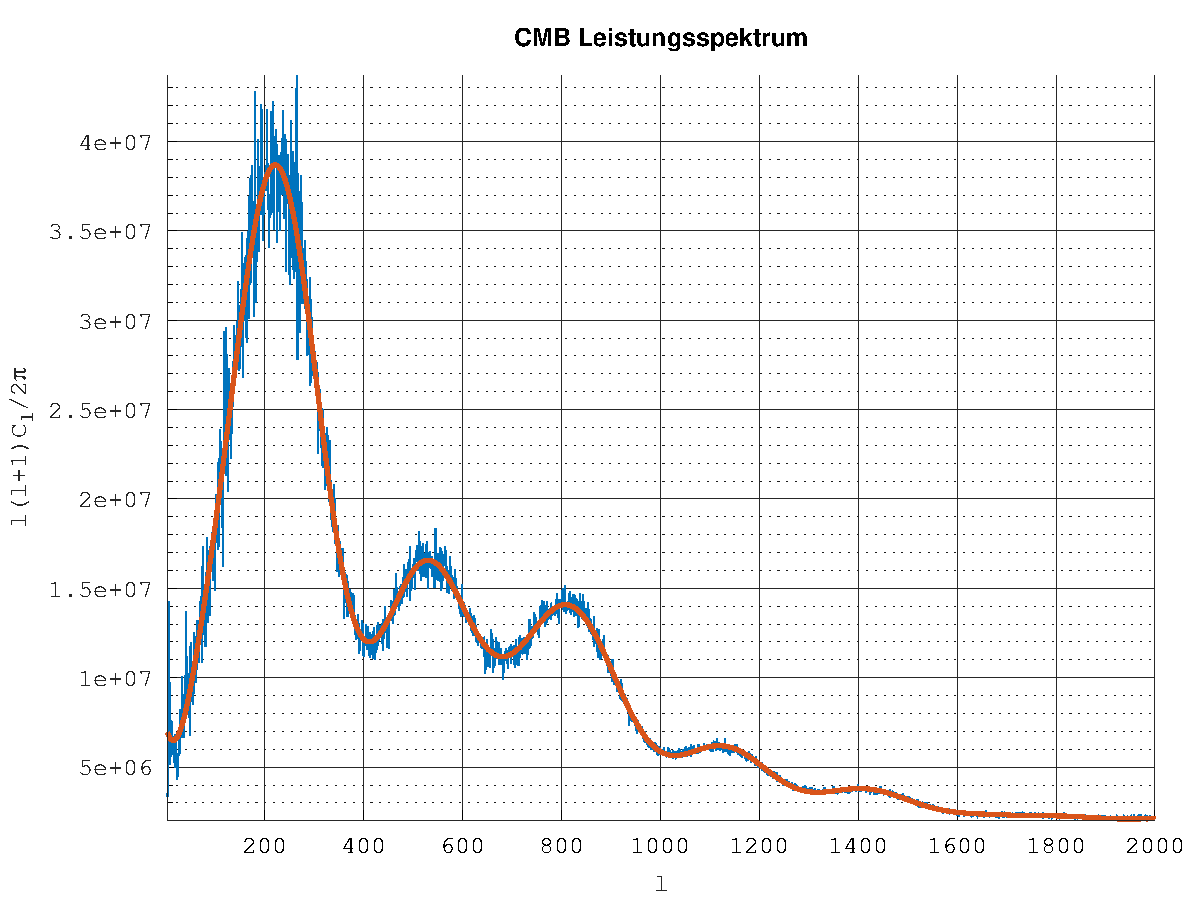
\includegraphics[width=\linewidth]{cmb/data/12k2500-500.pdf}
	\caption{Leistungsspektrum berechnet bis zu $l = 2100$. Grundlage für die 
	Berechnung ist das 12K aufgelöste Bild der ESA Planck Mission.}
	\label{fig:cmb-power-spec-2000}
\end{figure}
